\documentclass[10pt]{article}
\usepackage[margin=0.8in]{geometry}
\usepackage{amsmath,amssymb}
\usepackage[T1]{fontenc}
\usepackage[utf8]{inputenc}
\usepackage{lmodern}
\usepackage{microtype}
\usepackage{booktabs}
\usepackage{enumitem}
\usepackage{graphicx}
\usepackage[hidelinks]{hyperref}
\hypersetup{pdftitle={Where the Galaxy Law Sets the Core}}
\setlist{nosep,leftmargin=1.3em}
\setlength{\parskip}{3pt}\setlength{\parindent}{0pt}
\sloppy
\begin{document}
\begin{center}
{\Large\bfseries Where the Galaxy Law Sets the Core:\\ $a_0$ and the Structure of Cold Dark Energy Halos,\\ from Galaxies to Clusters}\\[6pt]
{\small Working note, 2026-10-25, v1.0 (draft 1). AI-assisted research programme; not peer reviewed. $\kappa=\tfrac12$ is fitted; the theory is not closed.}
\end{center}

\begin{abstract}\noindent
The owner's programme studies a galaxy law, $g_N=g^2/(g+a_0)$ with $a_0=c^2\sqrt{\Lambda/32\pi}$ ($\kappa=\tfrac12$ fitted), and its covariant form v3s. This note follows the record's lanes from that law to what lies beyond it, on both $a_0$ footings ($9.36\times10^{-11}$ and $1.13\times10^{-10}$\,m\,s$^{-2}$, never pooled).
\begin{enumerate}
\item \textbf{The law} passes the SPARC radial-acceleration relation (rms 0.054\,dex), MeerKAT's $a_0$, isolated groups, tidal dwarfs, the screened Solar System and binary pulsars.
\item \textbf{Beyond galaxies} it fails. Cluster cores sit above it at $Z$ 4.1--5.5. Faint dwarfs carry a real, mass-driven extra. The early universe needs a cold component that is already dust-like by $z\approx5\times10^4$. We call that component \emph{cold dark energy}: a gravitating $w\approx0$ field component paired with dark energy, not matter and not a particle.
\item \textbf{The doors that close.} Selectors, late or vacuum heating, feedback, early dark energy, recombination release and orbit-keyed conversion all fail, each with a named mechanism.
\item \textbf{Route E.} Cold dark energy is everywhere, and the law is the form it takes around baryons. The external-field test in the record does not distinguish a fundamental law from an emergent one.
\item \textbf{The core result.} Burkert cores with $\rho_0r_0=a_0/(2\pi G)$ (106.9 / 129.2\,$M_\odot$\,pc$^{-2}$, no new constant) pass SPARC and the cluster outskirts, but under-predict the heavy cluster cores. The rule $\Sigma_{\rm core}=\max(a_0/2\pi G,\ \eta\,\Sigma_{\rm coll})$, with $\eta=14.83$ from self-similar infall and an \emph{external} formation concentration $c_f=4$, passes SPARC and 14 of 15 cluster keys, including the heavy cores. It fails two keys narrowly: groups ($Z=+2.05$) and the gas-richest clusters' outskirts ($Z=+2.41$). $c_f$ is not yet derived; self-similar infall alone gives 1.85, which fails.
\item \textbf{A map, for orientation only.} A Cosmicflows-4 flow map with the SPARC galaxies and nearby eRASS1 clusters on it illustrates the picture. It is not evidence for the theory.
\end{enumerate}
\end{abstract}

\section{Setting and rules}
\begin{itemize}
\item $\kappa=\tfrac12$ is fitted. Footings: canonical $a_0=9.3603\times10^{-11}$, alternative $1.1312\times10^{-10}$\,m\,s$^{-2}$, never pooled; pairs below are canonical / alternative. Each lane froze its criteria before computing, ran a mutation control that must fail, and was rerun by the coordinator; the record's summary is \texttt{V3S\_FINAL\_VERDICT\_2026-10-24.md} (\S\S7--8) and \texttt{COLD\_SECTOR\_SPEC\_2026-10-24.md}. Lane folders are in \texttt{rebuild\_2026\_10\_22/}.
\item \textbf{Naming.} \emph{Cold dark energy} is the cold, clumping ($w\approx0$) component that the data require beyond the law. It is a gravitating field component paired with dark energy ($w\approx-1$). It is not matter and not a particle; ``dust-like'' describes only how it clusters. $\Lambda$CDM is the name of the external rival model.
\item No result here is evidence for the framework over $\Lambda$CDM or any other rival. Failures are stated with their mechanisms.
\end{itemize}

\section{The galaxy law}
In the static limit the law is AQUAL with $\mu(x)=x/(1+x)$, i.e.\ $g_N=g^2/(g+a_0)$, and $a_0=\kappa c\sqrt{G\rho_\Lambda}=c^2\sqrt{\Lambda/32\pi}$. Its covariant form, v3s, is a Khronon action with a switched stiffness term (PAPER60; the verdict, \S1). Its constraint algebra closes with 3 degrees of freedom, and the switched stiffness is well posed with the statics unchanged (qualifiers in the record). Table~\ref{tab:pass} lists what the law passes.

\begin{table}[h]\centering\small
\caption{What the galaxy law passes (canonical / alternative).}\label{tab:pass}
\begin{tabular}{p{0.27\textwidth}p{0.55\textwidth}l}
\toprule
test & result & lane\\
\midrule
SPARC radial acceleration & rms 0.054 / 0.054\,dex, one $\Upsilon$ per galaxy (median 0.52 / 0.44); the $\chi^2$ line fails, so conditional & P4\\
MeerKAT $a_0$ & $+0.032$\,dex from SPARC's, same recipe & P4\\
isolated groups & $+0.010$ / $-0.010$\,dex from the law on baryons & P4\\
tidal dwarfs & $+0.055\pm0.114$\,dex: Newtonian, as predicted & U1\\
Solar System (screened) & all 24 Cassini cells pass, by $4.8\times10^{7}$ to $5.1\times10^{9}$; the unscreened law fails & C6\\
binary pulsars & at most $3.2\times10^{-14}$ of the double pulsar's precision & C8\\
\bottomrule
\end{tabular}
\end{table}

As a theory of gravity and cosmology, v3s fails: clusters, growth and the CMB, the radiation era, hosted dwarfs and the Milky Way disc (PAPER60; verdict \S3). Most of these follow from one mechanism: v3s has one cold field, and kinematics fix it to be the field that carries the law. The rest of this note asks what lies beyond the law.

\section{What lies beyond galaxies}
\begin{itemize}
\item \textbf{Cluster cores.} In 0.3--1\,Mpc the cores sit 1.5--1.7 times above the law on their baryons. The statistical significance is $Z$ 4.5--5.5 (X11); after X13's correction for a shear-dependent source-size selection it is $Z$ 4.1--5.0, still real by X7's rule. Known baryons fall short by a factor 4--7 (X21).
\item \textbf{Small dwarfs: a real, mass-driven floor.} Against the isolated law, hosted dwarfs carry an extra that is not tidal and not binaries. The tidally safe subset ($\tau\le0.1$) still sits $+0.48$ / $+0.45$\,dex high, $Z=5.8$ / 5.4 (\texttt{X20\_hosted\_dwarf\_disequilibrium}). Being hosted adds nothing: field dwarfs of the same stellar mass carry the same extra. A velocity floor $\sigma^2=\sigma_{\rm iso}^2+c_0^2$, with $c_0=4.6$ / 4.1\,km\,s$^{-1}$ calibrated on field dwarfs only, cuts the hosted $\chi^2$ from 637 to 217 (canonical) and 559 to 195 (alternative) (X24). Tides at pericentre are ruled out: dwarfs with weak pericentric stress still sit $+0.60$ / $+0.55$\,dex high, $Z=4.8$ / 4.4 (X25). The floor is not in the action (\texttt{X25\_floor\_from\_action}).
\item \textbf{The early universe.} The Lyman-$\alpha$ forest needs dust-like clustering down to $\lambda_{\rm hm}\approx0.42$\,Mpc/$h$ ($M_{\rm hm}\approx4.9\times10^{9}\,M_\odot$). Gravity alone then drops the component into galaxies: median capture 0.76 of the fair share (X22). In patched CLASS, a cold component switched on at recombination is excluded ($\sigma_8$ at 0.050 / 0.047 of $\Lambda$CDM's for a turn-on at $z=1100$ / 1500). It must already be dust-like by $z\approx5\times10^4$ (X34).
\item \textbf{Its nature.} It must be collisionless and concentrated toward cluster centres. Any component added on top of the law, retained hydrostatically or partially, spreads mass outward: its predicted cluster OUTER band is 1.42--2.26 against measured $0.72\pm0.14$ / $0.66\pm0.13$ (X30). In the Bullet Cluster a dust-like tracer with dispersion near the well's survives ($f_{\rm ret}$ 0.80--1.02) and lands on the galaxies (X32).
\end{itemize}
In every test run in the record, the cold dark energy the data require behaves like the cold component of $\Lambda$CDM. No test here distinguishes it from that component. What the framework adds is the galaxy law, and with it the question of why isolated galaxies show no extra today.

\section{The doors that close}
Table~\ref{tab:doors} lists the mechanisms tried for keeping cold dark energy where the data want it, and how each fails.

\begin{table}[h]\centering\small
\caption{Doors tried for the cold sector (both footings unless noted).}\label{tab:doors}
\begin{tabular}{p{0.2\textwidth}p{0.6\textwidth}l}
\toprule
door & how it fails & lane\\
\midrule
one selector variable & no single catalogue variable or axis-aligned pair separates the classes that need extra from those that need none & X19\\
feedback energy & $F=e_{\rm fb}/\sigma^2$ does not order the classes (Spearman $+0.10$); the heavy clusters that need extra have the lowest $F$ & X31\\
universal late heating & clusters capture the whole fair share: $A_{\rm MID}$ 7.5--10.7 against 1.0--2.2 & X23\\
late heating, graded & hosted dwarfs get $\le8\times10^{-4}$\,dex against $+0.21$ to $+0.64$; clusters T2/T3 are over-captured & X23\\
vacuum heating & no $\epsilon$ window: the forest allows $\epsilon\le2.41\times10^{-6}$, SPARC needs $\ge7.65\times10^{-6}$ / $8.59\times10^{-6}$ & X24b\\
a heated sheet & survives the cluster terciles at 45 / 37 grid points, then all are excluded by the outskirts profile & X26, X30\\
early dark energy & UNDECIDED; v3s has nothing for a large early $a_0$ to act on ($\rho_\tau\equiv0$) & X35\\
recombination release & excluded at recombination; reduces to ordinary dust-like clumping by $z\approx5\times10^4$ & X34\\
orbit-keyed conversion & empties the cores first: OUTER 1.67 against $0.72\pm0.14$ ($Z=-6.7$); MID slope with KT of the wrong sign & X37\\
\bottomrule
\end{tabular}
\end{table}

The general statement (X37) is that any depletion rule keyed to orbits, density, temperature or time removes cold dark energy from cluster centres first, where the data want it most.

\section{Route E: the law as the form cold dark energy takes}
Route E puts cold dark energy everywhere, keeps gravity Newtonian, and reads the galaxy law as the form cold dark energy halos take around baryons. It inherits growth, the forest, the Bullet Cluster and the tidal dwarfs by construction.
\begin{itemize}
\item \textbf{With cusps it fails softly on SPARC (EM1).} NFW halos on one global SPARC halo-mass relation give rms 0.0656 but median $\Upsilon$ 0.36, below the stellar-population window. With $\Upsilon$ pinned at 0.5 for both, the dust model gives 0.1020 against the law's 0.1124 / 0.1029. SPARC alone does not separate them.
\item \textbf{The external field does not decide it (X36).} Large SPARC galaxies' residuals fall with the external field: slope $-0.561\pm0.175$ / $-0.525\pm0.176$. The law's own external-field effect predicts almost none of it ($Z=-3.21$ / $-2.99$). Route E reaches part of it ($Z=-2.26$ / $-2.06$). The two predictions differ by only 0.71 / 0.70 of the measurement's error, so the lane is NOT DIAGNOSTIC. Gaia DR4 wide binaries cannot separate them either: both readings predict Newtonian binaries.
\end{itemize}
\textbf{Stated plainly:} no test in the record yet distinguishes a fundamental law from a law that emerges from cold dark energy around baryons. In route E with cusps, the link $a_0\propto\sqrt\Lambda$ would be a coincidence. Section~\ref{sec:core} gives $a_0$ a role inside route E.

\section{The core surface density}\label{sec:core}
\textbf{X38: cores set by $a_0$.} Burkert-cored cold dark energy halos with $\rho_0r_0=a_0/(2\pi G)$, i.e.\ 106.9 / 129.2\,$M_\odot$\,pc$^{-2}$, add no new constant; galaxy halo masses use EM1's committed relation, and cluster halos take the fair share. SPARC passes at a sensible $\Upsilon$: rms 0.0795 / 0.0729, median $\Upsilon$ 0.77 / 0.60. The cluster OUTER band passes for the first time in the record (all-KT $Z=+0.14$ / $-0.06$), where every added-component model overshot. The heavy cores fail, under-predicted: MID T3 $Z=+4.26$ / $+3.80$, MID slope with KT $+3.07$ / $+2.99$, and the heaviest gas tercile's OUTER band (MGAS T3) $+5.36$ / $+4.94$. Its cluster cores come out too wide (0.44\,Mpc in the hottest tercile), and it also fails the groups line ($Z=+2.48$ / $+2.29$, X40b).

\textbf{What does not raise the cluster cores.}
\begin{itemize}
\item \textbf{Contraction (X39).} Blumenthal contraction by the BCG and hot gas moves MID T3 only from 1.05 to 1.13 against 2.13, and it rebuilds galaxy cusps: SPARC median $\Upsilon$ falls to 0.39 / 0.32 and fails. Any process that densifies cluster cores through baryons densifies galaxy cores first.
\item \textbf{A fixed core radius (X40).} The best SPARC value, $r_c=9.73$\,kpc, gives rms 0.119 at $\Upsilon$ 1.20 (fails), and overshoots the clusters.
\item \textbf{Framework-native rules (X40b).} Setting the core by $\max(a_0,g_b)$ never switches on: at cluster cores $g_b$ is only 0.04--0.07\,$a_0$. Setting it by $a_0$ at the formation epoch has the right sign but reaches at most a factor 1.34. With galaxies pinned, the clusters need $S\propto M^{\alpha}$ with $\alpha_{\rm best}=0.30$ / 0.25, i.e.\ cores at 3--5 times $a_0/(2\pi G)$.
\end{itemize}

\textbf{Collapse supplies the slope (X41).} The Lacey--Cole formation epoch on the record's own $P(k)$ gives the collapsed object's $\rho r$ a slope of 0.23 in mass over $10^{13}$--$10^{15}\,M_\odot$, close to the needed 0.25--0.30. Its amplitude is only 0.26 / 0.22 of $a_0/(2\pi G)$ at the cluster median, so a core-concentration factor $\eta$ of 11.4--19.0 / 13.8--23.0 is needed. X42 calibrated a self-similar rise on the cluster cores alone: it implies a factor of 9.0--14.4 over the same collapse $\rho r$, and it fails the groups out of sample ($Z=+2.41$ / $+2.27$).

\textbf{X43: floor plus collapse core.}
\[
\Sigma_{\rm core}(M)=\max\!\left(\frac{a_0}{2\pi G},\ \eta\,\Sigma_{\rm coll}(M)\right),\qquad \eta=\frac{4}{3B(1)}\,c_f^{5/4}=14.83\quad[c_f=4\ \text{EXTERNAL}].
\]
Cold dark energy collapses like collisionless dust (Bertschinger's self-similar infall, $\rho\propto r^{-9/4}$); its core is the inner $1/c_f$ of the half-mass object at the Lacey--Cole formation epoch; and it can never be cored more thinly than the floor $a_0/(2\pi G)$. Nothing is fitted; $c_f=4$ is an external value from collapse studies. The crossover falls at $M\approx10^{12.1}$ / $10^{12.4}\,M_\odot$: galaxies sit on the $a_0$ floor, groups and clusters on the collapse core. Table~\ref{tab:core} shows the grades.

\begin{table}[h]\centering\small
\caption{Core rules graded on the same keys (canonical; alternative in brackets where it differs in class). Measured MID T3 2.13, MGAS T3 OUTER 1.37. X44 sets $c_f$ from self-similar infall timing.}\label{tab:core}
\begin{tabular}{lllll}
\toprule
key & X38 (floor only) & X43 ($c_f=4$, external) & X43, $c_f=5$ (reported) & X44 ($c_f=1.85$)\\
\midrule
SPARC rms / median $\Upsilon$ & 0.0795 / 0.77 & 0.0782 / 0.77 & 0.0721 / 0.72 & pass\\
groups $Z$ & $+2.48$ & $+2.05$ & $+1.82$ & $+2.48$ ($+2.29$)\\
MID T3 & 1.05, $Z=+4.26$ & 2.06, $Z=+0.30$ & --- & 1.40, $Z=+2.90$\\
MID slope with KT, $Z$ & $+3.07$ & $+1.70$ & --- & $+2.49$\\
MGAS T3 OUTER & 0.81, $Z=+5.36$ & 1.12, $Z=+2.41$ & fails & 0.95, $Z=+4.07$\\
cluster keys passing & 10 / 15 (11) & 14 / 15 & 14 / 15 & ---\\
\bottomrule
\end{tabular}
\end{table}

\textbf{What X43 passes and fails.} SPARC passes (rms 0.0782 / 0.0729, median $\Upsilon$ 0.77 / 0.60). The heavy cores pass: MID T3 moves from $Z=+4.26$ to $+0.30$ and the all-MGAS OUTER band from $+2.36$ to $+0.49$. Two keys fail, both slightly under-predicted: groups at $Z=+2.05$ on both footings (line 2.0), and the MGAS T3 OUTER band, 1.12 against 1.37 ($Z=+2.41$). Reported only, not adopted: $c_f=5$ ($\eta=19.6$) passes the groups ($Z=+1.82$).

\textbf{The status of $c_f$.} It is external, and two keys fail; X43 is not a pass. A first derivation from scale-free self-similar infall timing (X44) gives $c_f=2^{8/9}=1.85$ ($\eta=5.66$), which fails four keys: groups, MID T3, the MID slope and MGAS T3 OUTER. The data pin $c_f\approx4$--4.2: X43's groups line crosses $Z=2.0$ at $c_f\approx4.21$ / 4.20, and X42's cluster-only calibration gives 3.3--4.6. That is the standard formation concentration. It needs the structure of the initial density peaks and cannot come from scale-free infall; the framework does not derive it.

\textbf{Reading.} The cold dark energy core surface density is $a_0/(2\pi G)$ in galaxies. Above galaxy scale it is the collapse value raised by a formation concentration. In this picture $a_0=c^2\sqrt{\Lambda/32\pi}$ is a constant of the cold sector, and the galaxy law is what the $a_0$ floor looks like. $\kappa$ is still fitted, and adopting the picture is the owner's decision, not a lane result.

\section{The cosmic river map (illustrative)}
\begin{figure}[t]\centering
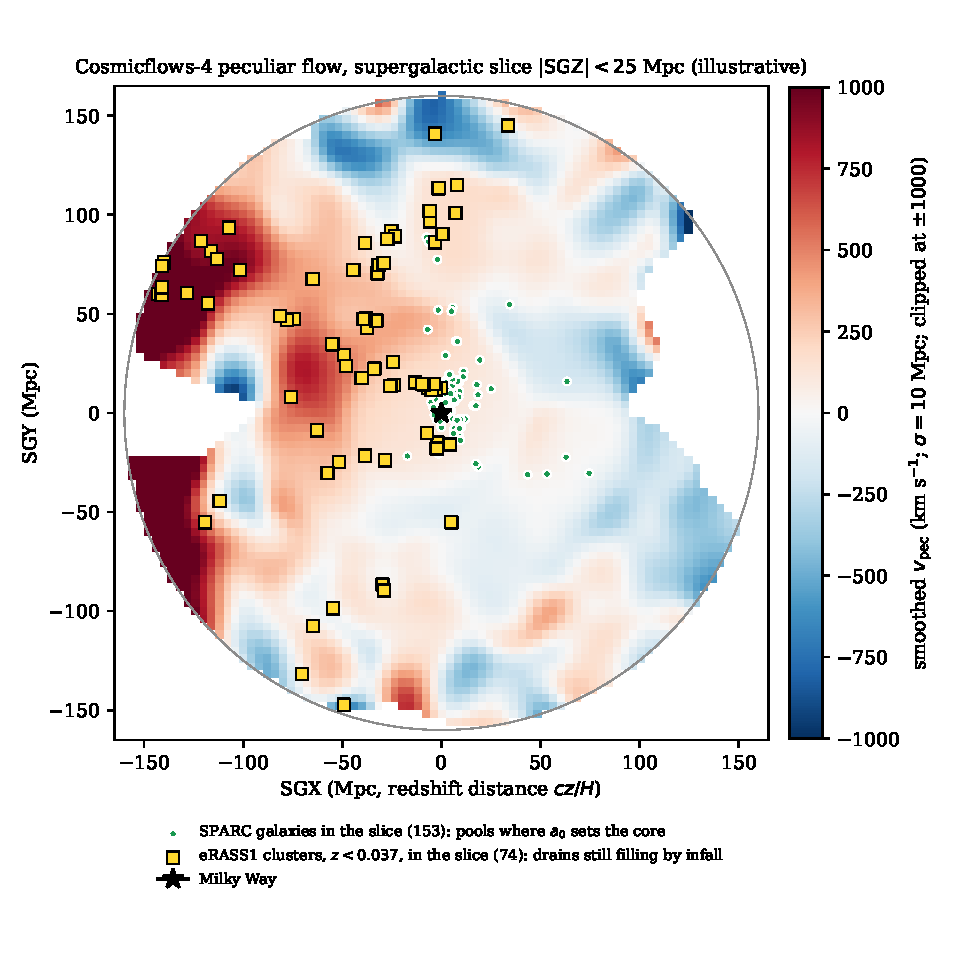
\includegraphics[width=0.72\textwidth]{PAPER61_fig_river.pdf}
\caption{Measured Cosmicflows-4 peculiar flow in the supergalactic slice $|{\rm SGZ}|<25$\,Mpc, $R<160$\,Mpc (MAP1). Colour: smoothed peculiar velocity ($\sigma=10$\,Mpc kernel, inverse-variance weights, shown where at least 3 effective groups contribute), clipped at $\pm1000$\,km\,s$^{-1}$; red recedes faster than the Hubble flow. Green dots: SPARC galaxies in the slice, labelled ``pools where $a_0$ sets the core''. Yellow squares: eRASS1 clusters at $z<0.037$ in the slice, labelled ``drains still filling by infall''. The labels are the reading of Section~\ref{sec:core}, not measurements. Illustrative only: the map is not evidence for the theory.}\label{fig:river}
\end{figure}
Figure~\ref{fig:river} places the two regimes of Section~\ref{sec:core} on the measured local flow. MAP1 groups the 38,035 Cosmicflows-4 galaxy groups, self-calibrates $H=73.56$\,km\,s$^{-1}$\,Mpc$^{-1}$ on the catalogue's own distance scale, and computes peculiar velocities with the Watkins--Feldman estimator. The slice holds 5,875 groups, 153 SPARC galaxies (at X33's distances) and 74 of the 178 eRASS1 clusters within 160\,Mpc. No fit is made and no verdict is drawn.

\textbf{Caveats.} Per-group peculiar velocities are noisy (median error 905\,km\,s$^{-1}$). No inhomogeneous-Malmquist correction is applied, so the field at large $R$ is biased. eRASS1 covers only the western Galactic hemisphere, so the cluster positions trace the survey footprint as much as the cosmic web. The map shows where the two regimes sit; it tests nothing.

\section{Discussion}
\textbf{Open.}
\begin{itemize}
\item \textbf{Fundamental or emergent?} No test in the record separates a fundamental law from a law that emerges from $a_0$-cored cold dark energy (X36, EM1).
\item \textbf{The origin of $c_f$.} The one external number in X43. It is pinned by the data at $c_f\approx4$ but not derived in the framework: scale-free infall gives 1.85 and fails (X44). A derivation would have to start from the structure of the initial peaks.
\item \textbf{The two failing keys.} The groups and the gas-richest clusters' outskirts are both under-predicted. A first-principles $c_f$ of 4--5 would close the groups; the MGAS T3 OUTER band also failed X40b's power law, X42's two rules and X43, so it is not specific to one rule. The verdict asks for a data-side check of that band before more rules are built on it.
\item \textbf{What lies outside the picture.} The dwarf floor $c_0$ is a separate, undetermined constant; the mechanism that keeps cold dark energy at the $a_0$ floor in galaxies is not an action; and nothing here is a cosmology.
\end{itemize}

\textbf{Data still to come} (dated, sealed before the data): the Khronon-native L1 $512^3$ growth run (in the compute queue; the converged ladder says the nonlinear hold term does not restore growth); ALMA U4 (2026-11-06) and GS4 (2026-11-28); Gaia DR4 wide binaries and the Milky Way (2026-12-02).

\section{What this is not}
\begin{itemize}
\item Not closed: $\kappa$ is fitted; $c_f=4$ is external; the groups and MGAS T3 OUTER keys fail.
\item Not evidence for the framework over $\Lambda$CDM or any other rival. The cold dark energy required here behaves, in every test run, like the cold component of $\Lambda$CDM.
\item No particle species is added: cold dark energy is a gravitating field component.
\item The river map is illustrative, not a test.
\end{itemize}

\textbf{Disclosures.} X43's criteria were frozen at 00bc1a7950 with no amendment; one loader path fix preceded the first graded run. X44's result (66273956b2) was committed while this note was drafted; it is folded into the verdict (58a2d738f8, coordinator rerun identical apart from timing) and into \texttt{COLD\_SECTOR\_SPEC\_2026-10-24.md}. Its 4.21 / 4.20 crossing is in its \texttt{.out}; the 3.3--4.6 range is in its README and the verdict, not its JSON. X38's groups failure was found in X40b, not X38. X42's H1 has one cluster-calibrated amplitude, so its SPARC pass is by construction. X24 is post hoc and disclosed in its lane. The verdict document's ``107 / 129'' is $a_0/(2\pi G)$ rounded; the JSON gives 106.9 / 129.2. Two references (Watkins \& Feldman 2015; Lacey \& Cole 1993) are cited by name from the lanes and are not in the record's bibliography.

\section{Data and code availability}
{\footnotesize
All lanes are in \texttt{rebuild\_2026\_10\_22/}; commits are criteria / result. Galaxy law: P4 (6c5e6161b9 / 6c0249a8bc), with U1, C6, C8 as in PAPER60. Beyond galaxies: X11 (9a105431c9 / c1cd5455a5), X13 (c4e5a5a064 / 4eeeceba07), X21 (a48f6d5e08 / 3aa4f07b58), \texttt{X20\_hosted\_dwarf\_disequilibrium} (87b6832e84 / bd736c128e), X24 (7a79903c3f / 19d31a99d9), X25 (d4827bece5 / 5a754eb2e2), X22 (a2b532e3c6 / 5c7114f508), X34 (6c5d581400 / ab4a3a8e1a), X30 (c6be83f91c / 0f19b6759b), X32 (57ff3e7df4 / 975ccfbf49). Doors: X19 (8960ea2285 / a9ec701f5b), X31 (1aa11f9bcb / 358e3859ed), \texttt{X23\_late\_heated\_cold} (b8d81770bb / df896db507), \texttt{X23\_late\_heating\_graded} (6ec6b89807 / 9c54fae62e), X24b (1d0f8c6967 / 3492bcbeb4), X26 (b10263968f / c9112e3126), X35 (02848d0330 / 0eb84a459a), X37 (204001f8ad / 538dc083c9). Route E: EM1 (1b0dbd6eef / 889d65276e), X36 (d8651cafc3 / 8d7df6a74d). Core: X38 (9cc80516df / 3e28ca3027), X39 (b75acfc767 / 54684fb62f), X40 (b37983a0f7 / 5dc30a7c1a), X40b (b09db13390 / ba368d2ba1), X41 (0ea05957ee / e9c1b9abe4), X42 (4a13086d02 / 0d7d0d5686), X43 (00bc1a7950 / bf8cc9e7cf), X44 (c8dd02f5aa / 66273956b2). Map: MAP1 (3f9b3ae361). Summaries: \texttt{covariant\_push\_2026\_10\_22/V3S\_FINAL\_VERDICT\_2026-10-24.md}, \texttt{COLD\_SECTOR\_SPEC\_2026-10-24.md}. This note: \texttt{PAPER61\_fig\_river.py} (the figure, from MAP1's JSON) and \texttt{PAPER61\_core\_audit.py} (every number checked against its lane's JSON, \texttt{.out} or README; a mutation mode that must fail). Companion: PAPER60 (doi:10.5281/zenodo.23601528).
Data: F.~Lelli, S.~S.~McGaugh, J.~M.~Schombert, AJ 152, 157 (2016) (SPARC); R.~B.~Tully et al., ApJ 944, 94 (2023) (Cosmicflows-4); E.~Bulbul et al., A\&A 685, A106 (2024) (eRASS1).
Theory: E.~Bertschinger, ApJS 58, 39 (1985); J.~A.~Fillmore, P.~Goldreich, ApJ 281, 1 (1984); A.~Burkert, ApJ 447, L25 (1995); C.~Lacey, S.~Cole (1993); R.~Watkins, H.~A.~Feldman (2015).
AI assistance: Anthropic's Claude (lanes, review, drafting).}
\end{document}
